\section{Проверка работоспособности приложения}

Осуществлялось функциональное тестирование, ниже рассмотрим тестирование каждой функции.

1 Тестирование функции регистрации – ожидаемый результат, появление нового пользователя в 
таблице базы данных при передаче уникального имени, соответствует полученному.

2 Тестирование функции авторизации – ожидаемый результат, предоставление валидного токена авторизации, 
соответствует полученному.

3 Тестирование функции просмотра категорий – ожидаемый результат, получения списка категорий, соответствует полученному.

4 Тестирование функции просмотра информации о пользователе – ожидаемый результат,
 получение объекта, описывающего пользователя, соответствует полученному.

5 Тестирование функции просмотра лотов определенной категории – ожидаемый результат, получения списка объектов данной категории, соответствует полученному.

6 Тестирование функции удаления категории – ожидаемый результат, удаление из таблицы базы данных категории пользователем в роли администратора, 
соответствует полученному.

7 Тестирование функции просмотра лотов определенного пользователя – ожидаемый результат, получения списка объектов лотов данного пользователя, соответствует полученному.

8 Тестирование функции просмотра собственных лотов – ожидаемый результат, получения списка объектов лотов данного 
авторизованного пользователя, соответствует полученному.

9 Тестирование функции просмотра ставок определенного пользователя – ожидаемый результат, получение списка объектов ставок, 
созданных даннным пользователем, соответствует полученному.

10 Тестирование функции изменение статуса лота – ожидаемый результат, 
измение поля ItemStatus в таблице базы данных, при выполнении запроса авторизованного пользователя с ролью администратора,
соответствует полученному.

11 Тестирование функции завершении аукциона – ожидаемый результат, изменение статуса лота в таблице базы данных
и уведомление пользователей в режиме реального времени, соответствует полученному.

12 Тестирование функции создания лота – ожидаемый результат, создание новой сущности в таблице базы данных 
при передаче корректных данных и извещение администратора, соответствует полученному.
Ниже на рисунке 4.1 показан результат, полученный в программном средстве Postman.
\begin{figure}[h]
\centering
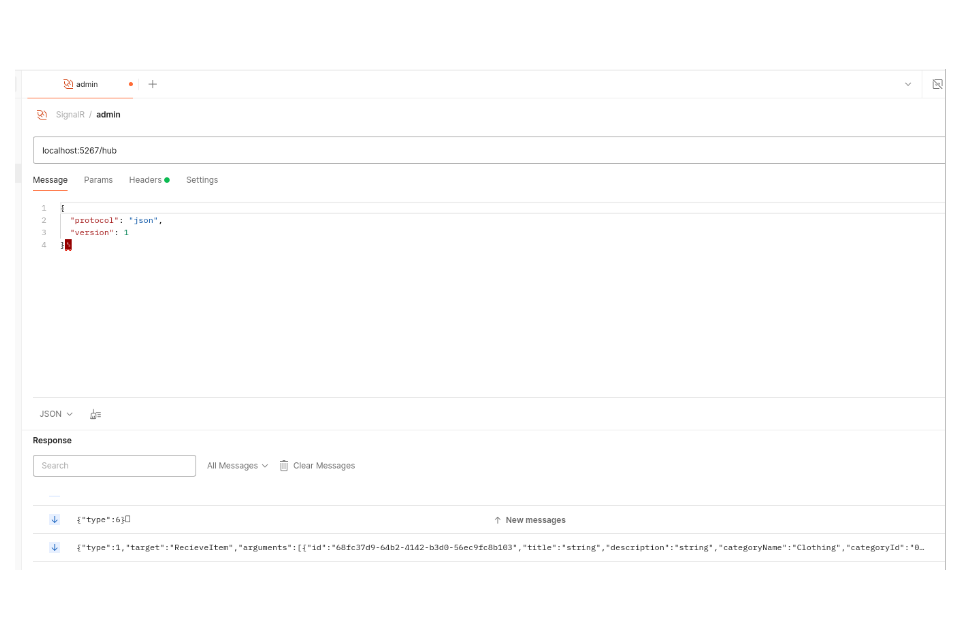
\includegraphics[scale=0.3]{test11.png}
\caption{Тестирование уведомления администратора при создании нового лота}
\end{figure}

13 Тестирование функции удаления лота – ожидаемый результат, удаление соответствующей сущности из таблицы в базе данных , соответствует полученному.

14 Тестирование функции изменения лота – ожидаемый результат, изменение сущности в таблице базы данных при 
передаче корректных данных и извещение администратора об изменении, соответствует полученному.
Ниже на рисунке 4.2 показан результат, полученный в программном средстве Postman.
\begin{figure}[h]
\centering
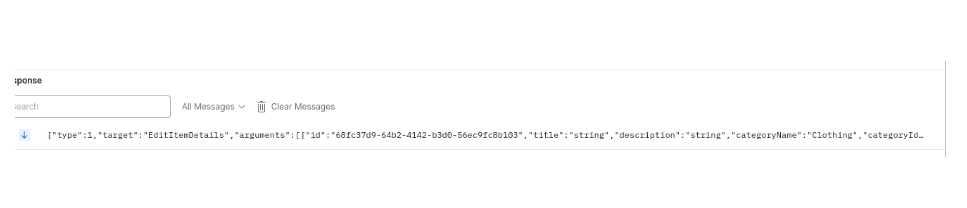
\includegraphics[scale=0.3]{test22.png}
\caption{Тестирование уведомления администратора при изменении лота}
\end{figure}
% 15. Тестирование функции просмотра ставок определенного лота – ожидаемый результат, получения списка объектов ставок определенного лота, соответствует полученному.

% 16. Тестирование функции создания ставки – ожидаемый результат, 
% добавление новой ставки в таблицу базы данных при достаточной сумме взноса, 
% соответствует полученному.
% На рисунке 4.3 показан результат уведомления в программном средстве Postman.

% \begin{figure}[h]
% \centering
% 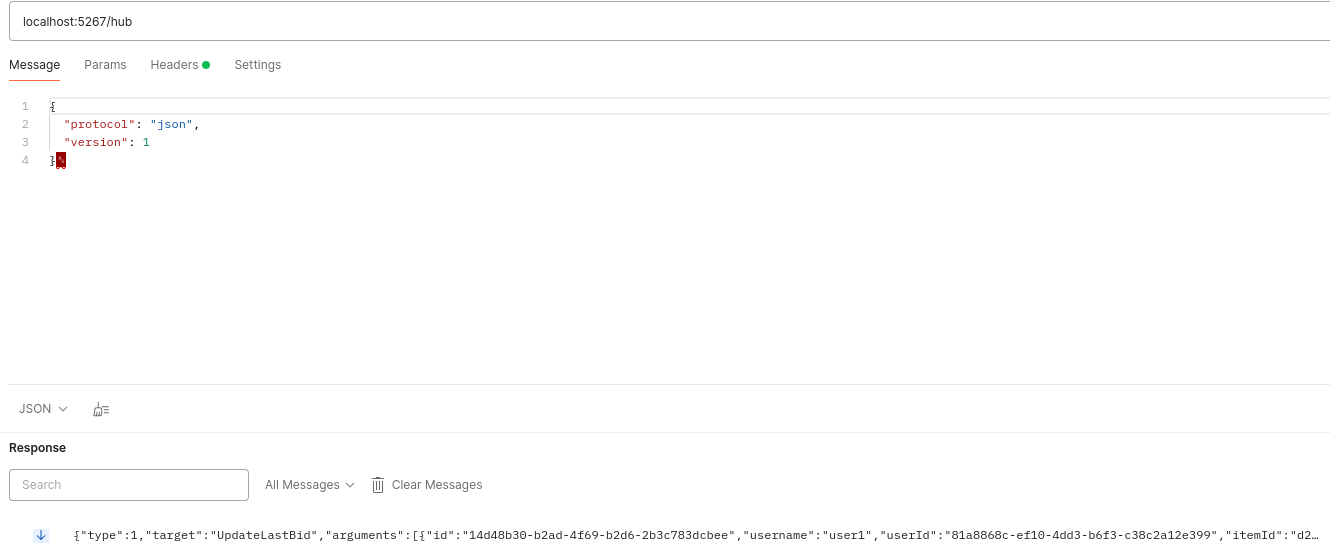
\includegraphics[scale=0.3]{test3.png}
% \caption{Тестирование уведомления администратора при создании ставки}
% \end{figure}
Таким образом, на основе выполненных тестов модно сделать вывод о том, 
что программное средство работает исправно и готово к дальнейшему использованию.